\documentclass[sigconf,nonacm]{acmart}
\settopmatter{printacmref=false,printfolios=true}
\setcopyright{none}
\renewcommand\footnotetextcopyrightpermission[1]{}
\usepackage{amsmath,tabularx,array,enumitem,balance}
\definecolor{CourseBlue}{HTML}{315EFB}
\definecolor{CourseTeal}{HTML}{14877D}
\hypersetup{
  colorlinks=true,
  linkcolor=CourseBlue,
  citecolor=CourseTeal,
  urlcolor=CourseTeal
}
\newcolumntype{Y}{>{\raggedright\arraybackslash}X}
\setlist{leftmargin=*,topsep=3pt,itemsep=2pt}
\newcommand{\CourseNumber}{COMSCI/ECON 206}
\newcommand{\CourseName}{Computational Microeconomics}
\newcommand{\CourseSession}{Autumn 2026 Session 1}
\newcommand{\Instructor}{Luyao Zhang}
\newcommand{\WorkshopSession}{Session G --- Promises, Deception, and Coordination}
% Personal project links for the submitted PS1 repository.
\newcommand{\GitHubLink}{%
  \href{https://github.com/qingyueliu/PS1-Qingyue}%
  {GitHub project repository}%
}
\newcommand{\TemplateRepository}{%
  \href{https://github.com/dku-comsci-econ206-Autumn2026/ps1-overleaf-template}%
  {class PS1 template}%
}
\newcommand{\ColabLink}{%
  \href{https://colab.research.google.com/github/qingyueliu/PS1-Qingyue/blob/main/companion/notebooks/strategic_reporting_qlearning.ipynb}%
  {Open the reproducible notebook in Colab}%
}
\newcommand{\DemoLink}{%
  \url{https://huggingface.co/spaces/dku-comsci-econ206-2026/qingyue}%
}

\newcommand{\coursemeta}{%
  \noindent\textbf{Submission to:} \CourseNumber{} --- \CourseName.\\
  \textbf{Course session:} \CourseSession.
  \textbf{Workshop:} \WorkshopSession.\\
  \textbf{Instructor:} \Instructor.
  \textbf{Assignment:} PS1 research proposal.\par\smallskip
}
\title{When Honest Reports Fail to Sustain Cooperation}
\author{Qingyue Liu}
\affiliation{
  \institution{Duke Kunshan University}
  \city{Kunshan}
  \country{China}
}
\email{ql186@duke.edu}
\renewcommand{\shortauthors}{Qingyue Liu}

\begin{document}
\begin{teaserfigure}
\captionsetup{skip=8pt}
\centering
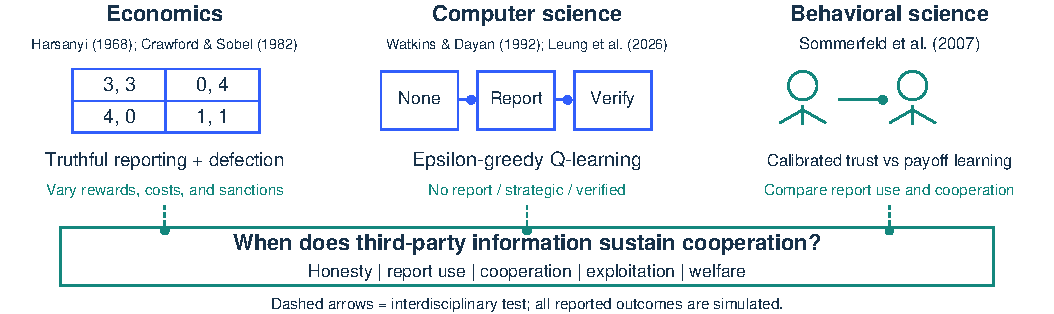
\includegraphics[width=\textwidth]{figures/ps1_teaser.pdf}
\caption{Research design for third-party reports in a repeated Prisoner's
Dilemma. An incomplete-information benchmark~\cite{harsanyi1968,crawford1982},
a Q-learning comparison~\cite{watkins1992,leung2026}, and competing behavioral
explanations for trust~\cite{sommerfeld2007} converge on one test: whether
truthful, accurate, or verified information changes cooperation and welfare.
Dashed arrows mark the proposed interdisciplinary synthesis.}
\Description{Three editable Draw.io panels show a Prisoner's Dilemma payoff
matrix, four information conditions for learning agents, and a receiver deciding
whether to trust a third-party report. Dashed arrows connect the panels to a
shared evaluation of cooperation, report use, exploitation, and social welfare.}
\label{fig:teaser}
\end{teaserfigure}
\maketitle\raggedbottom\coursemeta
\noindent\textcolor{CourseTeal}{\footnotesize
\textbf{Template and artifacts.}
This individual proposal adapts the \TemplateRepository; project links and
verification appear in Section~5.}\par\smallskip

\section{Three connected research questions}
Minimal third-party observation can help learning agents find cooperative partners~\cite{leung2026}, but a strategic observer may send false, incomplete, or unverifiable reports. In my application, C observes B's previous action, reports it to A, and A decides whether to use the report before playing B. Marketplaces, AI-agent platforms, and public allocation systems face the same tension. Figure~\ref{fig:teaser} connects three questions:

\textbf{Q1---Economics:} Which rewards, lying costs, or verification rules make C's report credible and welfare improving?\par
\textbf{Q2---Computation:} Can Q-learners identify useful reports and sustain cooperation across information conditions?\par
\textbf{Q3---Behavior:} Does report use reflect calibrated trust, or ambiguity and short-run optimism?

Together they ask when institutions can turn third-party information into calibrated trust without creating a new channel for manipulation.

\section{Answer to Q1: incentives and intellectual lineage}
After round 1, C observes B's action $s\in\{C,D\}$ in a preceding C--B exposure stage and sends $m\in\{C,D\}$; A uses or ignores $m$, then A and B simultaneously cooperate or defect. A/B payoffs are $(3,3),(0,4),(4,0),(1,1)$; C gets $h=0.4$ for truth and pays $\ell=0.2$ for lying. Truth strictly benefits C, but defection improves A's or B's payoff by one against either opposing action. A Bayesian-Nash benchmark~\cite{harsanyi1968} can therefore combine truthful reporting with mutual defection. This matches strategic-communication theory: informativeness depends on aligned incentives, not message availability alone~\cite{crawford1982}.

\textbf{Hypothesis.} Increasing $\ell$ raises honesty but not cooperation. Verification helps only if information changes a consequential margin such as partner selection, future access, or sanctions. The welfare benchmark is A+B payoff, separating credible reporting from socially useful reporting.

\section{Answer to Q2: method and evaluation}
The browser baseline uses tabular Q-learning~\cite{watkins1992}: $\epsilon=0.12$, action $\alpha=0.12$, $\gamma=0.85$, with reporter $\alpha_C=0.15$, $\gamma_C=0.80$. Recorded unseeded simulations produced 85.0\%, 3.8\%, and 0.7\% mutual cooperation over 100, 10,000, and 100,000 rounds; honesty stayed near 94\%, while welfare fell from 5.68 to 2.46 and 2.27.

Across 30 fixed seeds and 10,000 rounds, cooperation is 3.29\% without reports and below 3\% in every reporting treatment; strategic honesty is 93.98\%. Exact means and dispersion appear in Appendix A. With truth dominant, $\epsilon$-exploration explains residual lies. Outputs are synthetic; next I add partner choice.

\clearpage\balance
\section{Answer to Q3: behavior and competing explanations}
Calibrated trust predicts that A uses reports that forecast realized behavior, consistent with evidence that gossip changes cooperation~\cite{sommerfeld2007}. A competing payoff-learning account predicts defection regardless of accuracy because defection dominates. If verification raises report use but not cooperation, while partner selection raises both, payoff learning is better supported. If accurate reports alone raise cooperation, trust has an independent role. Q-values are behavioral indicators, not felt trust, guilt, or belief. I would revise my claim if cooperation remained high in long seeded runs without consequences for reported information.

\section{Advanced development and future directions}
Nash, Harsanyi, and Selten received the 1994 economics prize for equilibrium analysis~\cite{nobel1994}; Harsanyi clarifies choice under unknown reliability. Sutton and Barto received the 2024 Turing Award for reinforcement learning~\cite{turing2024}. Today's boundary is that autonomous agents learn from other strategic agents' reports at machine speed. Integrating equilibrium incentives, learning dynamics, and behavioral trust explains why transparent information can remain ineffective.

\begin{table}[h]\caption{Roadmap from laureate foundations to contribution.}
\begin{tabularx}{\columnwidth}{@{}p{1.35cm}Y@{}}\toprule
\textbf{Horizon}&\textbf{Milestone and evidence}\\\midrule
Foundation&Equilibrium analysis and reinforcement learning.\\
PS1&Three-agent model, demo, seeded condition check.\\
Next&Add verification with partner selection.\\
Longer term&Validate with heterogeneous agents and people.\\
2056&Auditable allocation using calibrated information.\\\bottomrule
\end{tabularx}\end{table}

\noindent\textbf{Expected 2056 Nobel Prize and Turing Award contribution statement.}
By 2056, I aspire to develop auditable resource-allocation institutions that sustain cooperation when people, governments, and AI agents rely on strategic third-party information. Building on equilibrium analysis and reinforcement learning, I will integrate incentive design, reproducible multi-agent evaluation, and behavioral evidence to separate honesty, accuracy, verifiability, and social usefulness.

\subsection*{Open Science Statement}
\textbf{GitHub:} \GitHubLink\quad \textbf{Colab:} \ColabLink\par
The repository releases the LaTeX source, editable figure, standard-library model, notebook, saved synthetic outputs, tests, and browser game. Run \texttt{python companion/src/strategic\_reporting.py}. Submitted commit: \textbf{5c87056}. Student code uses the MIT License; other materials retain their terms.

\subsection*{Statement of Contribution to the UN's SDGs}
\textbf{Hugging Face:} \DemoLink\par
The open-access game supports \textbf{SDG 4---Quality Education}~\cite{sdg4}: students vary information and incentives, compare outcomes, or play as A to learn why honesty and cooperation differ. A pre/post explanation question can measure the intended learning outcome; improvement has not yet been evaluated.

\clearpage\nobalance
\section*{Author Notes}
\subsection*{Acknowledgements}
I thank Prof. Luyao Zhang, Program Chair, and Prof. Ken Rogerson, Program Discussant, of the \emph{2056 Nobel and Turing Laureate Program Launch Workshop}, held at Duke Kunshan University on September 7, 2026. I also thank Feiyu Li and Yitong Lin, my teammates in Session G, \emph{Promises, Deception, and Coordination}, and the rest of the COMSCI/ECON 206 Autumn 2026 Session 1 class for their questions and discussion. Preparing the session alongside their work on economic credibility and computational deception detection helped me distinguish incentives from trust and detection. I am responsible for the proposal and remaining errors.

\subsection*{Individual contribution}
I framed the A--B--C reporting game, selected its payoff and information structure, specified the intrinsic honesty reward and lying cost, designed and tested the Week 2 browser demonstration, interpreted the recorded outputs, and revised the research questions. I adapted the course ACM/Overleaf template and its editable-figure structure. AI assistance used for drafting, debugging, and formatting is disclosed below; I checked the game rules, calculations, source links, and evidence labels.

\bibliographystyle{ACM-Reference-Format}\bibliography{references}

\appendix
\section{Technical details and reproducibility}
The browser baseline uses A and B payoffs $(3,3)$, $(0,4)$, $(4,0)$, and $(1,1)$. Except in round 1, each period begins with a C--B exposure interaction. C observes B's exposure-stage action, reports it, and then A and B play the focal interaction. C receives $+0.4$ for truth and $-0.2$ for lying. Action Q-learning uses $\alpha=0.12$, $\gamma=0.85$, and $\epsilon=0.12$; reporter learning uses $\alpha_C=0.15$ and $\gamma_C=0.80$. Reported cooperation, exploitation, and welfare measure the focal A--B interaction; exposure-stage payoffs are not included in the welfare statistic. Restarting clears scores and Q-values. The Hugging Face Space is static HTML/CSS/JavaScript with no API, database, backend, secret, paid service, or hosted CPU/GPU runtime.

The earlier browser outputs were unseeded single runs. The PS1 notebook supplies a deterministic Python reconstruction using seeds 0--29 and 10,000 rounds per seed. It compares no report, strategic report, verified report, and a higher lying cost. Run \texttt{python companion/src/strategic\_reporting.py}; the saved output is in \texttt{companion/outputs/ps1\_condition\_panel.json}. Unit tests check the payoff table, strict dominance of defection, repeatability by seed, and condition labels. The reconstruction mirrors the demonstration's learning rules, but it is not a reproduction of Leung et al.'s population and partner-selection model~\cite{leung2026}.

\begin{table}[h]
\caption{Seeded PS1 synthetic check: means over 30 seeds and 10,000 rounds.}
\begin{tabularx}{\columnwidth}{@{}Yrrrr@{}}\toprule
Condition & Coop.\% & Honest\% & Used\% & Welfare\\\midrule
No report & 3.29 & -- & -- & 2.38\\
Strategic & 2.75 & 93.98 & 43.60 & 2.38\\
Verified & 2.39 & 100.00 & 100.00 & 2.36\\
High lie cost & 2.75 & 93.98 & 43.60 & 2.38\\\bottomrule
\end{tabularx}
\end{table}

Across-seed SDs for cooperation are 3.74, 1.62, 1.83, and 1.62 percentage points in table order. Thus the panel supports the limited claim that all four conditions converge toward low cooperation under the stated learning rule; it does not establish that verification causally lowers cooperation. The code and saved output retain additional dispersion statistics for audit.

\subsection{AI-use disclosure}
I used ChatGPT 5.6 Sol on August 30, September 5, and September 9, 2026 to organize my proposal, revise wording, create and debug the browser simulation, and synthesize cumulative worksheet responses. On September 13, 2026, I used OpenAI Codex with GPT-5.6 Sol to adapt the course LaTeX template, draft the five-section PS1 structure from my existing work, generate a seeded standard-library Python reconstruction, prepare an editable Draw.io teaser, and audit the draft against the instructor's grading criteria. I retained my independently chosen research question, A--B--C mechanism, payoff structure, and interpretation that honesty alone did not sustain cooperation. I rejected treating simulated Q-values as human mental states or finite-seed mean gaps as causal effects, and labeled new outputs as synthetic. I reviewed the wording and remain responsible for every claim, citation, and computation. Initial reasoning, handwritten reflections, and peer reviews remain Human-Only.

\section{Cumulative Intellectual Development}
This proposal develops my Intellectual Statement II through the \emph{2056 Nobel and Turing Laureate Program Launch Workshop}, held on September 7, 2026 at Duke Kunshan University, IB 2050. Program Chair: Prof. Luyao Zhang. Program Discussant: Prof. Ken Rogerson. My session was Session G, \emph{Promises, Deception, and Coordination}; my role was Speaker 3 and behavioral-science contributor. My teammates were Feiyu Li and Yitong Lin.

My Week 1 claim treated reports mainly as true or false. Field observations and the CodeCarbon and OpenFisca examples led me to distinguish honesty from accuracy, completeness, and verifiability. Preparing Session G separated three mechanisms: Feiyu Li's economics contribution emphasized incentive credibility, Yitong Lin's computer-science contribution emphasized detecting planned deception, and my behavioral-science contribution emphasized strategic uncertainty. On September 9, the longer simulation runs challenged my expectation that high honesty would preserve cooperation: honesty remained near 94\%, while cooperation and welfare fell. I therefore changed the proposal from ``does lying destroy cooperation?'' to ``when does credible information become behaviorally useful?'' and added controlled information conditions and a social-planner welfare benchmark.

My earlier aspiration was to develop a game-theoretic allocation system that is fair, efficient, sustainable, and difficult to manipulate. The revised statement narrows the unresolved boundary to auditable allocation when decisions depend on strategic third-party information. Appendix~\ref{app:abstract} records the current version; earlier Week 1--3 files are preserved separately.

\section{Field and open-source inspiration}
I attended the \emph{Joint Interdisciplinary Field Trip---Technology, Computation, Culture \& Society in Action} on September 4, 2026 and recorded the following observations.

\begin{figure}[h]
\centering
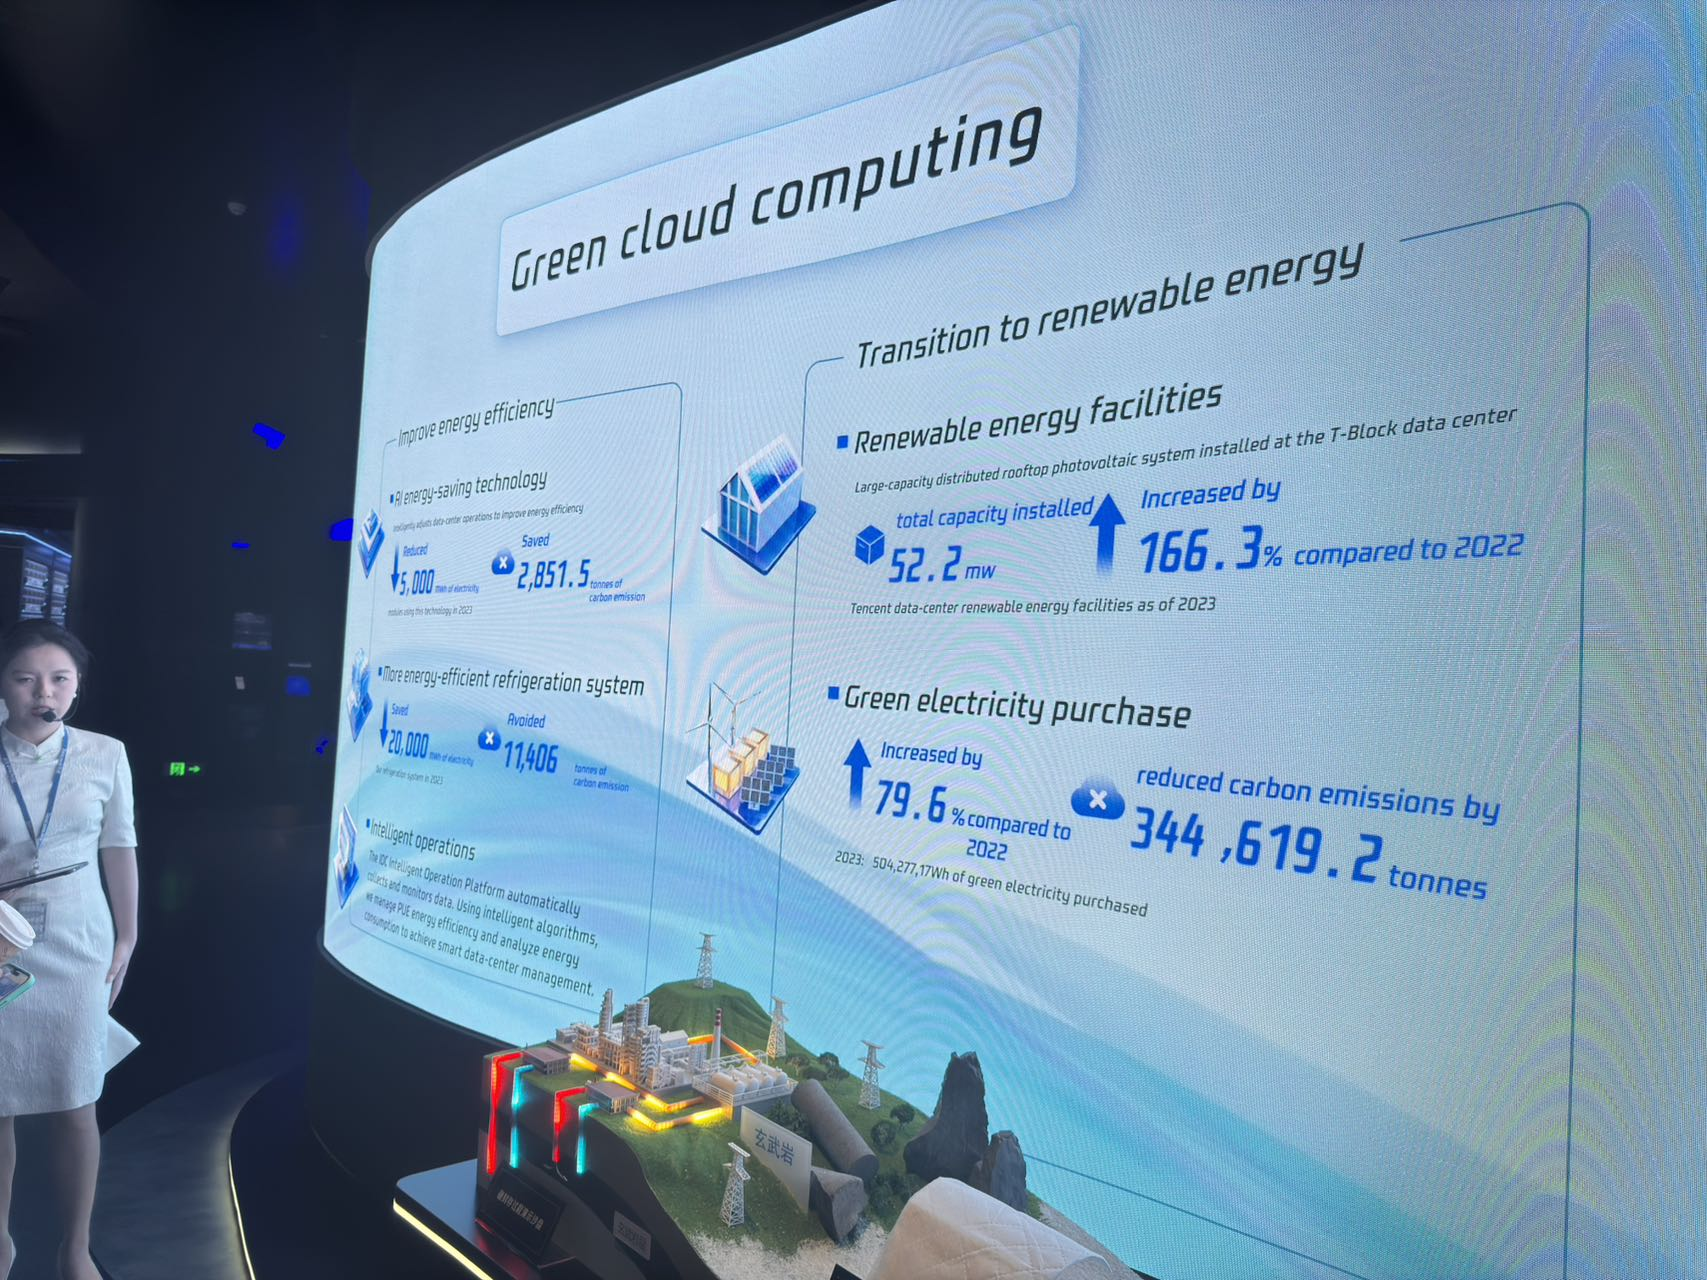
\includegraphics[width=\columnwidth]{figures/field/tencent_green_cloud.jpeg}
\caption{Tencent Shanghai Office, September 4, 2026. Photograph by Qingyue Liu. Direct observation: a display reported green-cloud energy and emissions measures. Interpretation: decision makers need auditable evidence, but quantified reports may still be incomplete. CodeCarbon inspired separating reported measurements from their coverage limits.}
\Description{A Tencent exhibit screen titled Green cloud computing displays renewable-energy capacity, electricity purchase, energy savings, and reported carbon-emission reductions.}
\end{figure}

\begin{figure}[h]
\centering
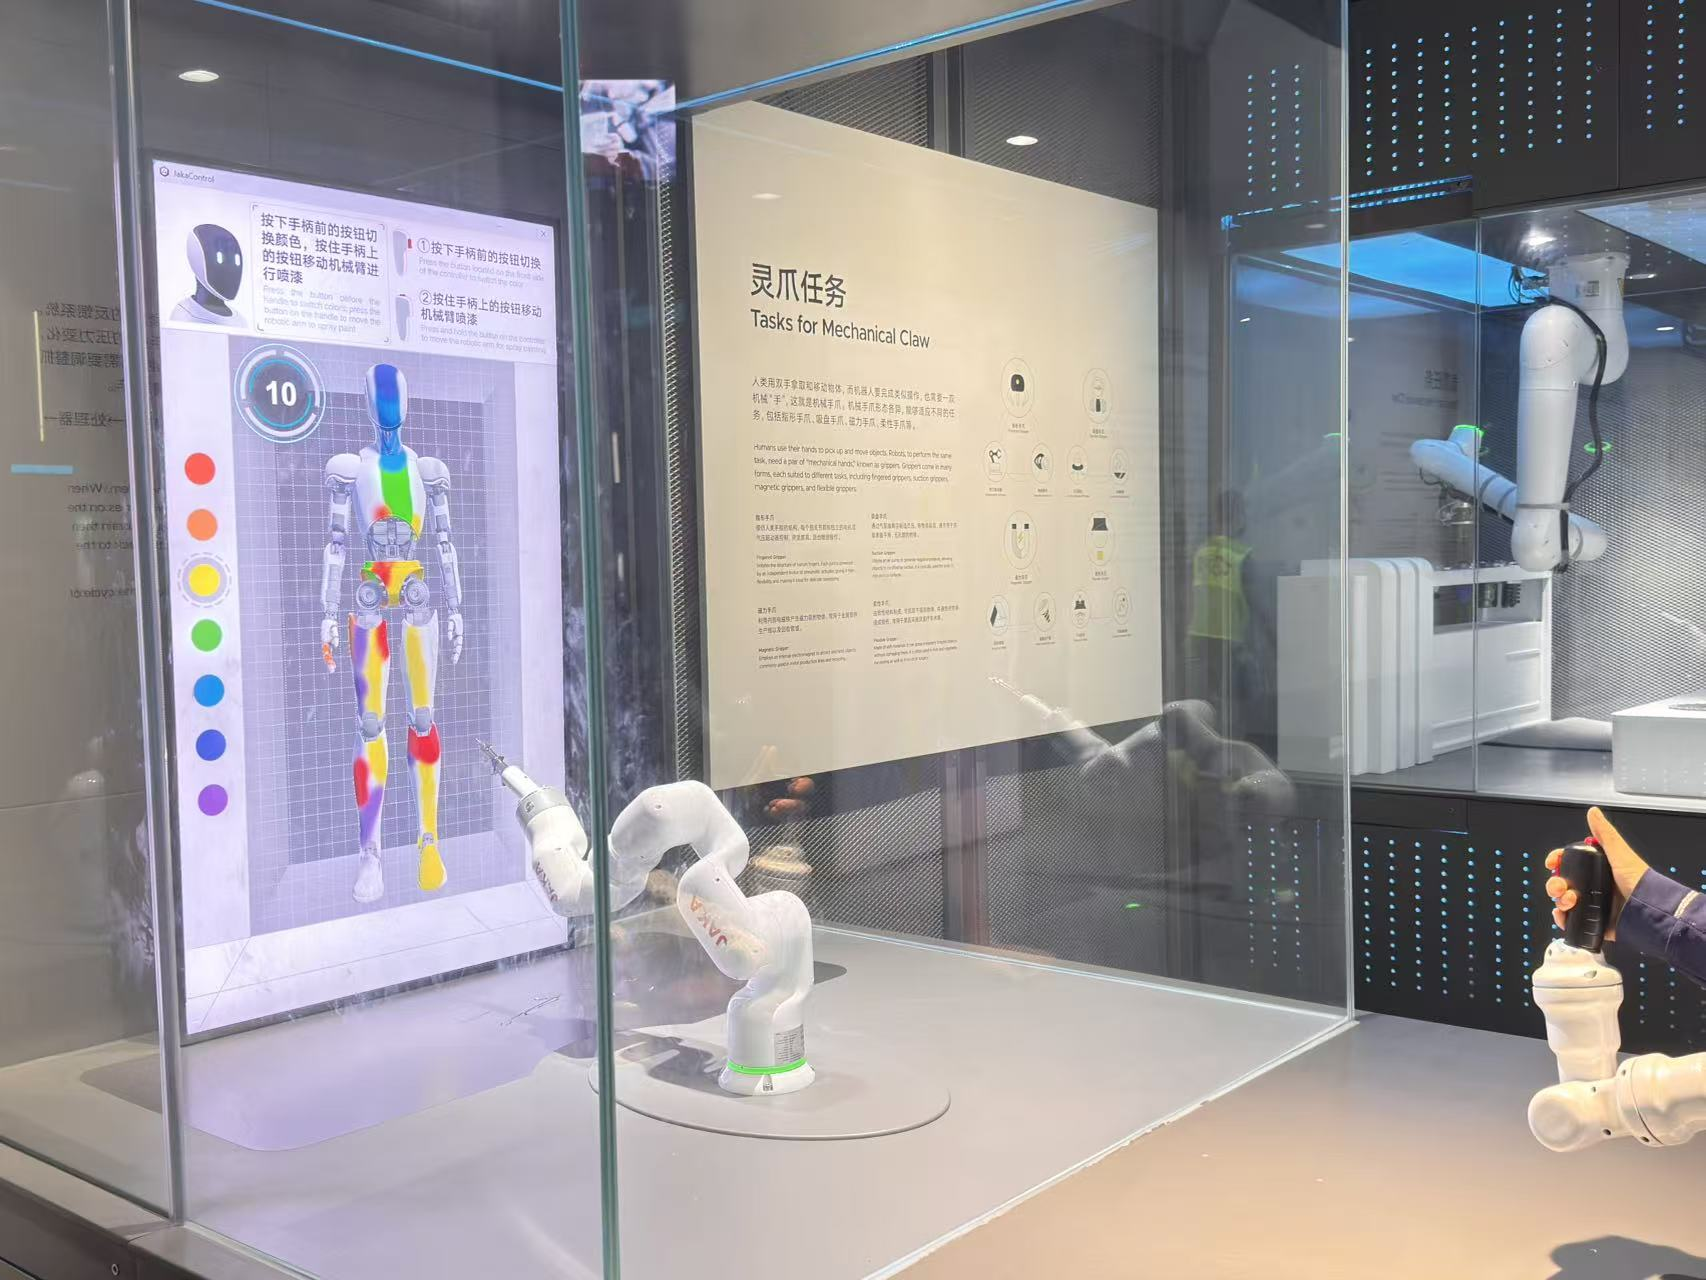
\includegraphics[width=\columnwidth]{figures/field/museum_mechanical_claw.jpeg}
\caption{Shanghai Science and Technology Museum, September 4, 2026. Photograph by Qingyue Liu. Direct observation: visitors could control a mechanical claw. Interpretation: interactive experience can communicate a mechanism more clearly than reported numbers alone. This observation motivated the playable Agent A mode and the SDG 4 learning use.}
\Description{A visitor operates a joystick beside an enclosed mechanical-claw exhibit with an instructional screen and robotic arms.}
\end{figure}

CodeCarbon 3.3.0 estimates computing energy and carbon emissions but omits some network, storage, and cooling components~\cite{codecarbon}; this motivates honest-but-incomplete reports. OpenFisca 44.7.0 converts policy rules into executable models but depends on correct rules and inputs~\cite{openfisca}; this motivates explicit institutional rules and a social-planner benchmark. These are inspirations, not software dependencies of the PS1 simulation.

\section{Review response and revision record}
This is the preserved v1 draft for class review on September 14, 2026. Two peer reviews, the author rebuttal, reviewer follow-up, and v2 are pending and are not invented here. After review, I will record each consequential concern, the section or notebook cell changed, the rerun performed, and whether the evidence resolved the concern.

\clearpage\onecolumn
\section{Structured abstract and cumulative proposal map}\label{app:abstract}
Table~\ref{tab:abstract-map} updates the eight-row cumulative proposal map while preserving earlier Week 3 files.
\par\medskip
\begin{table}[H]
\caption{Appendix E structured abstract and cumulative proposal map.}
\label{tab:abstract-map}
\renewcommand{\arraystretch}{1.18}
\begin{tabularx}{\textwidth}{@{}p{0.24\textwidth}Y@{}}
\toprule
\textbf{Proposal element} & \textbf{Current statement / change} \\
\midrule
Background & Minimal third-party observation can support cooperation among learning agents~\cite{leung2026}, but existing models do not establish what happens when an observer strategically reports information that may be false, incomplete, or unverifiable. \\
Motivation and application & Reputation systems, AI-agent platforms, marketplaces, and public allocation depend on reports about potential partners. The project asks when those reports improve decisions rather than create a manipulable information channel. \\
Three connected questions & Economics asks which incentives and verification rules make reports welfare improving; computer science asks whether Q-learners use them effectively; behavioral science asks whether report use reflects calibrated trust or competing mechanisms. Integrated question: when does credible information become behaviorally useful? \\
Method and model assumptions & C observes B's previous action and may report truthfully or lie; A uses or ignores the report; A and B play a repeated Prisoner's Dilemma. A seeded Q-learning panel compares no report, strategic report, verified report, and a higher lying cost, tracking cooperation, honesty, report use, exploitation, and welfare. \\
Results or expected results & Obtained browser simulations showed cooperation falling from 85.0\% at 100 rounds to 0.7\% at 100,000 rounds while honesty stayed near 94\%. The seeded PS1 check found 2.75\% cooperation under strategic reporting and 2.39\% under verification, but the across-seed dispersion means this gap is descriptive, not a causal verification effect. Planned partner-selection tests could challenge the conclusion by making accurate reports consequential. \\
Intellectual merits & The proposal connects incomplete-information incentives, reproducible reinforcement learning, and behavioral trust. It distinguishes honesty, accuracy, verifiability, and usefulness, showing why reliable messages need not change a dominant-action outcome. \\
Practical impacts & The model can inform reputation and audit rules in private and public allocation. The open-access game supports an intended SDG 4 learning activity; pre/post explanations of the honesty--cooperation distinction provide a feasible evaluation indicator. \\
Feedback received and revision made & September 4 field evidence and open-source tools exposed incomplete reporting; September 7 Session G preparation separated credibility, detection, and strategic uncertainty; September 9 simulation results rejected my expectation that high honesty would sustain cooperation. I added controlled comparisons, a social-planner benchmark, and explicit evidence labels. Peer-review feedback is pending. \\
\bottomrule
\end{tabularx}
\end{table}

\end{document}
